% !TEX root = main.tex
\chapter{Experiment}

Verifying the simulated aerodynamic effects is crucial to ensuring the correctness of the numerical analysis. In order to assess the reliability of the previouisly conducted simulations, a physical measurement of the pressure along the down-scaled wing.

In figure \ref{fig:scalewing} the down-scaled wing can be seen with pressure-taps along the centerpiece.

  \begin{figure}
    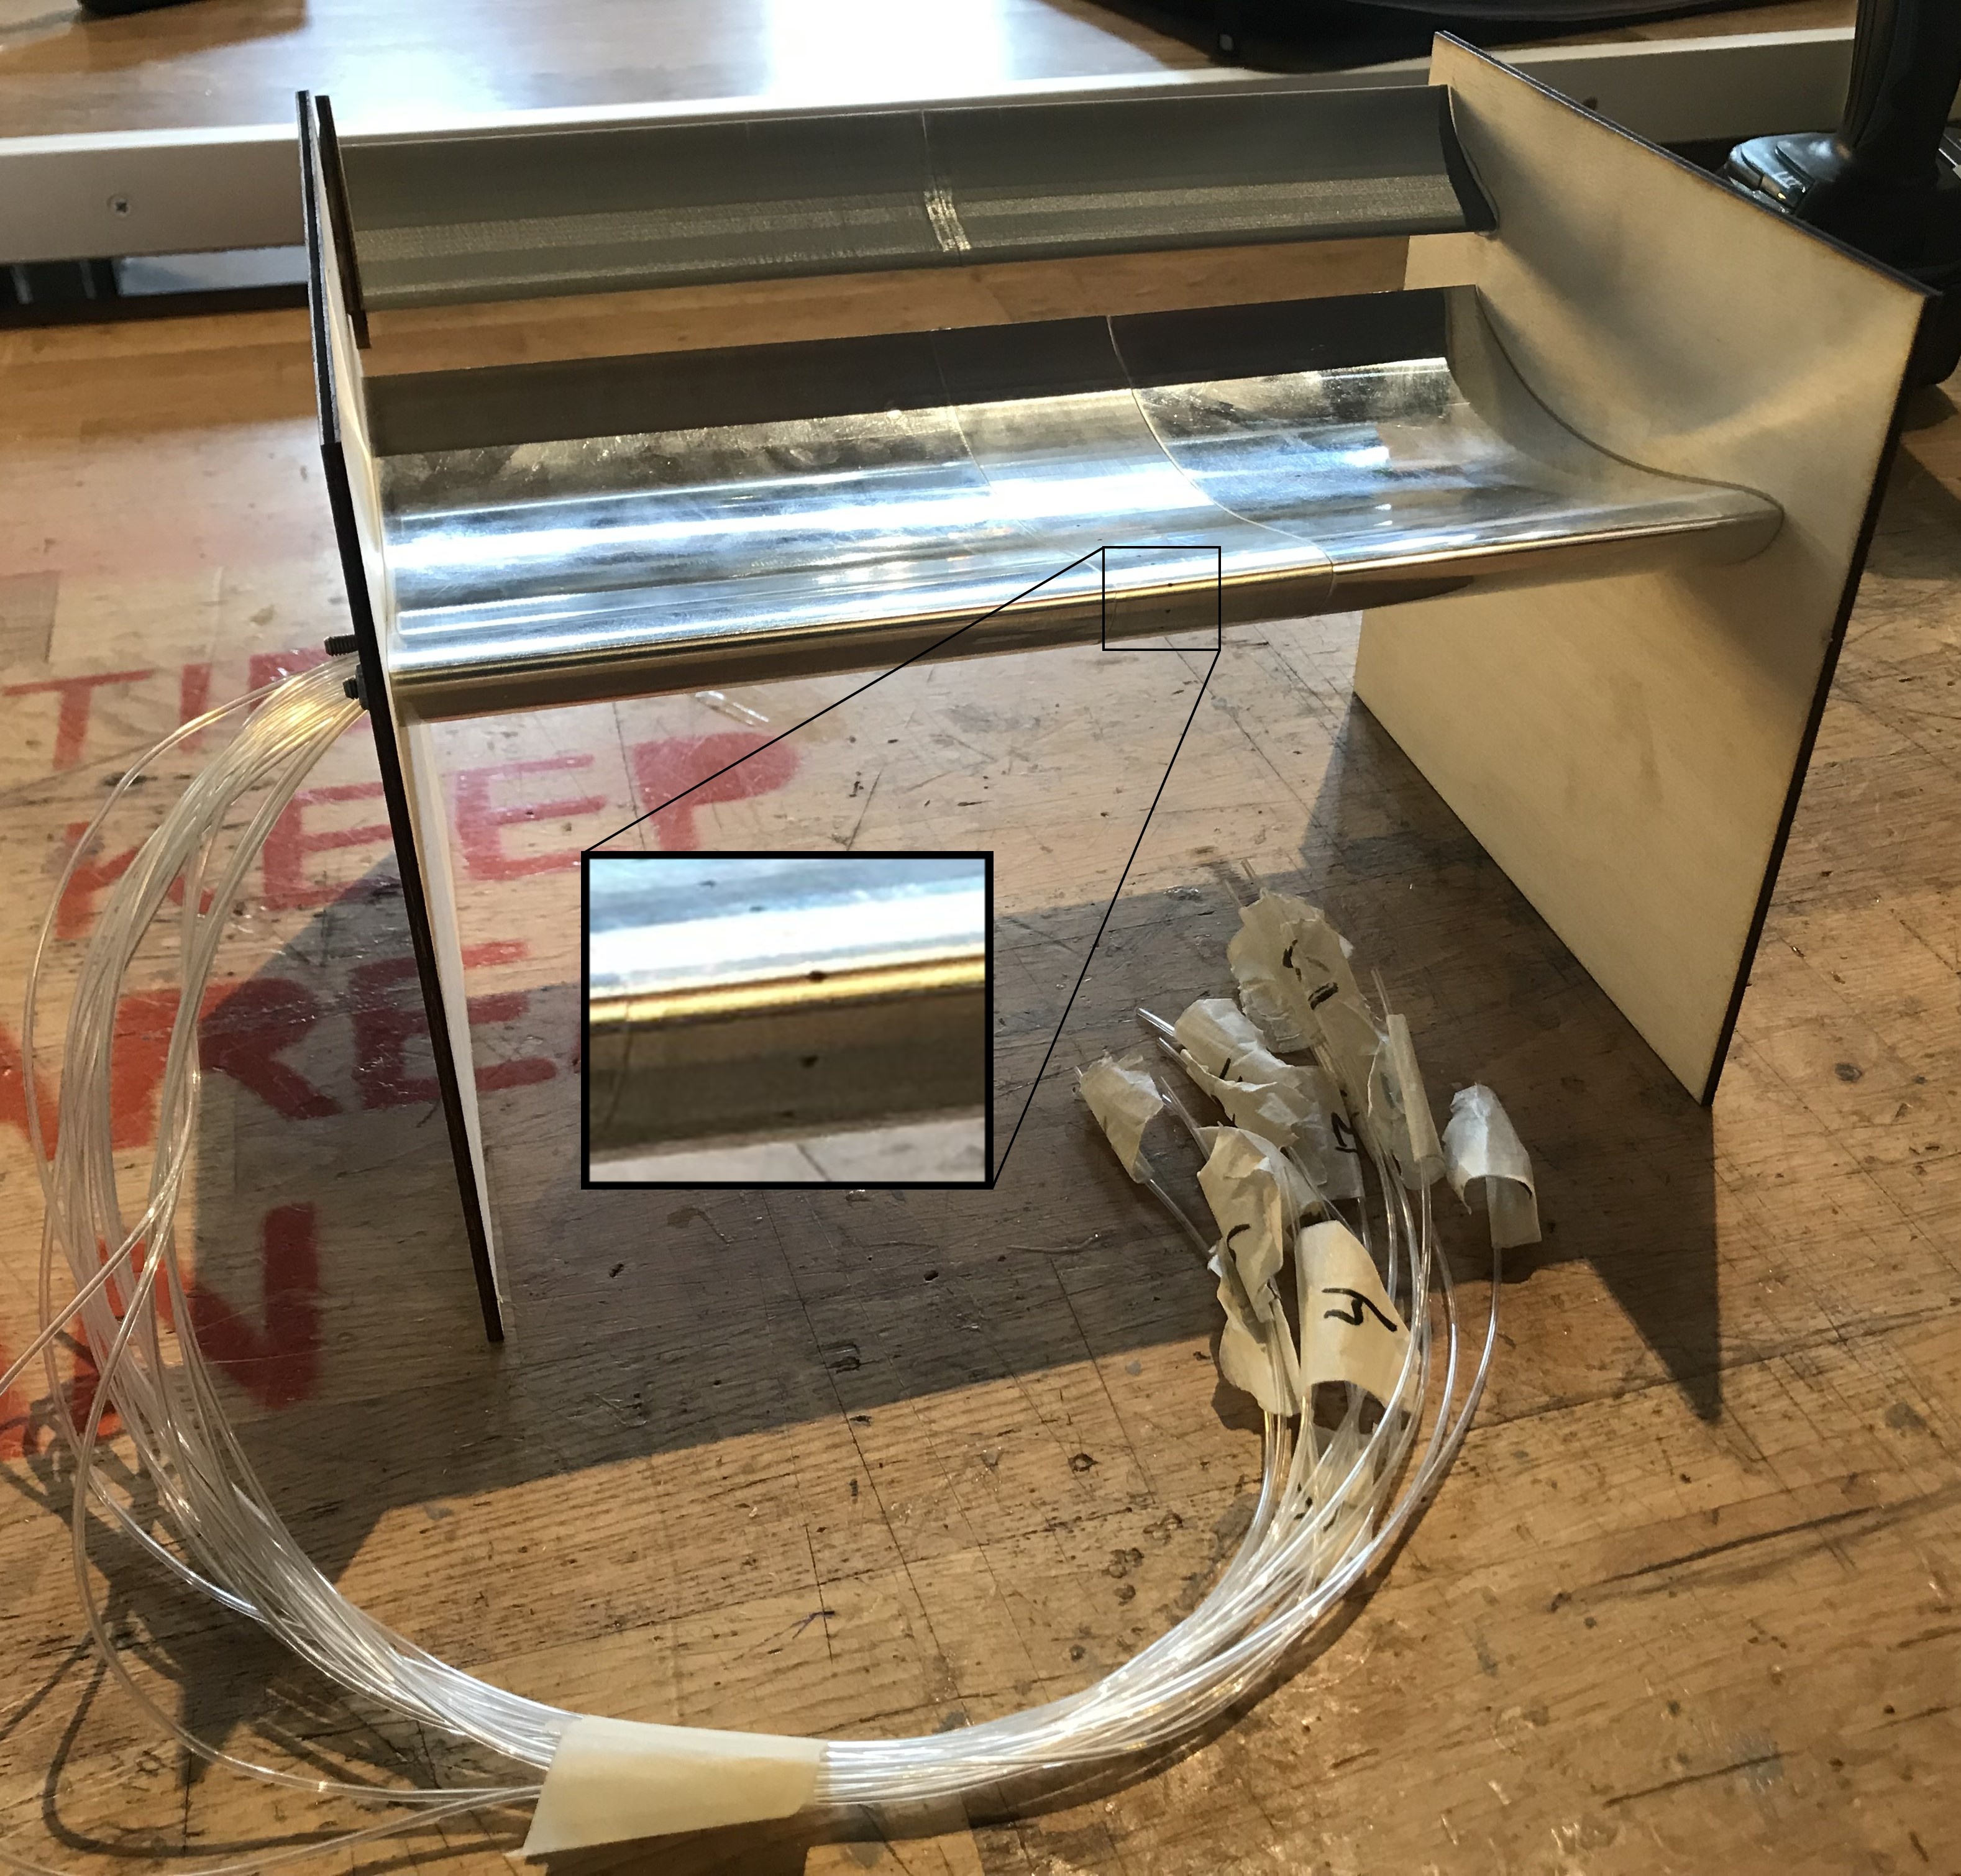
\includegraphics[width=\textwidth]{scalewingAssembled}
    \caption{Down-scaled wing assmembled with a zoom in on the pressure taps. The length of the entire wing is approximately $\SI{250}{\milli\metre}$ with a total chord length of $\SI{150}{\milli\metre}$.}
    \label{fig:scalewing}
  \end{figure}

\section{Aerodynamics}
  \subsection{Similarity of Flows}
  \label{sec:similarflows}

    In order to perform tests on the rear wing, it has to be scaled down to fit inside the wind tunnel. This reduces the physical size of the wing, which under equal circumstances changes the flow around it. In order to correctly emulate the simulated flow inside a wind tunnel, the Reynolds number and Euler number have to be the same, assuming incompressible flows:
    \begin{align}
      \text{Re}_\text{m} &= \text{Re}\\
      \text{Eu}_\text{m} &= \text{Eu}
      \intertext{Mathematically, the Reynolds- and Euler number are defined as:}
      \text{Eu} &= \frac{p_u - p_d}{pv^2}
      \intertext{where $v$ is the characteristic velocity of the flow, $p_u$ denotes upstream pressure, and $p_d$ denotes downstream pressure, and:}
      \text{Re} &= \frac{u L}{\nu}
    \end{align}
    where $u$ is the velocity relative to the object, $L$ is the characteristic length and $\nu$ is the kinematic viscosity of the fluid.

    For a down-scaled model, matching Reynolds- and Euler number requires an increase in velocity, inversely proportional to the increase in length \fxnote{skriv det her ud plx.}

    \begin{align}
      \frac{u_\text{m} L_\text{m}}{\nu} &= \frac{u L}{\nu} \nonumber \\
      \Rightarrow u_\text{m} &= \frac{L}{L_\text{m}} u \label{eq:windtunnelspeed}
    \end{align}


\section{Equipment}

  \begin{itemize}
    \item The Red wind tunnel ($\SIrange{60}{65}{\metre\per\second}$)
    \item 1/4 scale wing
    \item Syringe inserts
    \item Rubber tubing
    \item Pressure transducer
  \end{itemize}

  \subsection{1/4 Scale Wing}

    The small scale rear wing is constructed in 6 pieces. The large wing is dissected into three parts. Two regular wings, and a central part with 15 pressure taps.

    Material selection is based on the ease of machinability - a CNC-miller was provided to us, along with ample amounts of aluminium. This scale wing is not to be used in the actual race car, so weight is not a concern. Construction the 1/4 scale wing is not completely trivial. High precision is required for the surface finish, and the pressure taps have to be small in diameter: $Ø\SI{0.8}{\milli\metre}$. \fxnote{insert work drawings used for producing the wing}.

\section{Experimental Procedure}

Given the nature of the competition, the average cornering speeds are around $\SI{55}{\kilo \meter \per \hour} = \SI{15.28}{\metre\per\second}$, which is where downforce is of most importance. As shown in section \ref{sec:similarflows}, the desired velocity in the wind tunnel for the scale model can be found from equation \ref{eq:windtunnelspeed}

\begin{align*}
  u_\text{m} &= \frac{\SI{0.6}{\metre}}{\SI{0.15}{\metre}} \SI{15.28}{\metre\per\second} = \SI{61.12}{\metre\per\second}
\end{align*}

Which in accordance to the range of The Red wind tunnel.

\section{Results}
